\chapter{PLC State Machine Detailed Design and Flowcharts}
\label{ch:PLC-flowcharts}

		\section{Intraprogram Interfaces and Global Data}
		The Governor program interfaces with the Communications and motorControl programs via the two global scope variables, \textit{motorControl\_mode} and \textit{communications\_mode} which act as intraprogram interfaces. On each state transition, the Governor sets these variables  to certain values, determining what state to move the other programs into. The other programs can then set these variables to different values, informing the Governor on their own state changes and status which the Governor then uses as state transition conditions. Table ~\ref{table:progaminterfaces} shows the possible values of the intraprogram interfaces. 
		
		\begin{table}[htbp!]
			\begin{tabular}{|c|l|l|l|}
				\hline
				Code & motorControl\_mode & communications\_mode & Set By \\ \hline
				00 & Wait & Wait & Governor \\ \hline
				10 & Initialize & Ready & Governor\\ \hline
				11 & Initialization complete & Header received & motorControl/communications \\ \hline
				20 & Operate commands & Buffer command list & Governor \\ \hline
				21 & All buffered commands complete & Buffering complete & motorControl/communications\\ \hline
				22 & N/A & Buffer full & communications\\ \hline
			\end{tabular}
			\caption{Codes for interface between Governor, Communications and motorControl programs}
			\label{table:progaminterfaces}
		\end{table}
	
		In addition to locally scoped variables, there are also several key global scope variables that are used by two or more program that determine the behaviour and input of the system. These are shown in Figure ~\ref{table:globalvariables}

	\begin{center}
			\begin{tabular}{|l|l|p{10cm}|}
				\hline
				Variable Name & Element & Description\\ \hline
			%Spill over is included as a 'row', so use 4 instead of 2 for multirow
				\multirow{4}{*}{counterCommand} & .counter & Index number of the command currently being operated on by motorControl (also, how many commands have been processed)\\ \cline{2-3}
					 & .pointer & Index of where the command referred to by counterCommand.counter resides in the commandBuffer array\\ \hline
				\multirow{4}{*}{counterBuffer} & .counter & Index number of the command currently being buffered by Communications (also, how many commands have been buffered)\\ \cline{2-3}
					 & .pointer & Index of where the command referred to by counterBuffer.counter resides in the commandBuffer array\\ \hline
				\multirow{8}{*}{commandBuffer[]} & .command\_no & Command number of what the current array element stores\\ \cline{2-3}
					& .type & Determines the command type. 0 is a 'draw' and 1 is a 'move'. \\ \cline{2-3}
					& .x\_speed & For 'draw' operations, determines the X target speed for this sample. For 'move' operations, determines the target position for X to move to. \\ \cline{2-3}
					& .y\_speed & For 'draw' operations, determines the Y target speed for this sample. For 'move' operations, determines the target position for Y to move to. \\ \hline
				\multirow{8}{*}{boundaries} & .X\_CW & The number of clockwise steps from the center until the boundary in the X positive direction\\ \cline{2-3}
					 & .X\_CCW & The number of clockwise steps from the center until the boundary in the X negative direction\\\cline{2-3}
					 & .Y\_CW & The number of clockwise steps from the center until the boundary in the Y negative direction\\ \cline{2-3}
					 & .Y\_CCW & The number of clockwise steps from the center until the boundary in the Y positive direction\\ \hline
				\multirow{6}{*}{header} & .delta\_time & Period of velocity profile samples\\ \cline{2-3}
					 & .no\_commands & Total number of commands to be received and executed on\\ \cline{2-3}
					 & .max\_accel\_x & Max acceleration in the X axis\\ \cline{2-3}
					 &  .max\_accel\_y & Max acceleration in the Y axis\\ \cline{2-3}
					 & .move\_speed\_x & Target speed for 'move' operations in the X axis\\ \cline{2-3}
					 & .move\_speed\_y & Target speed for 'move' operations in the Y axis\\ \hline
			\end{tabular}
			\captionof{table}{Important global scope variables used by multiple programs}
			\label{table:globalvariables}
		\end{center}


\section{Governor}

		\begin{center}
				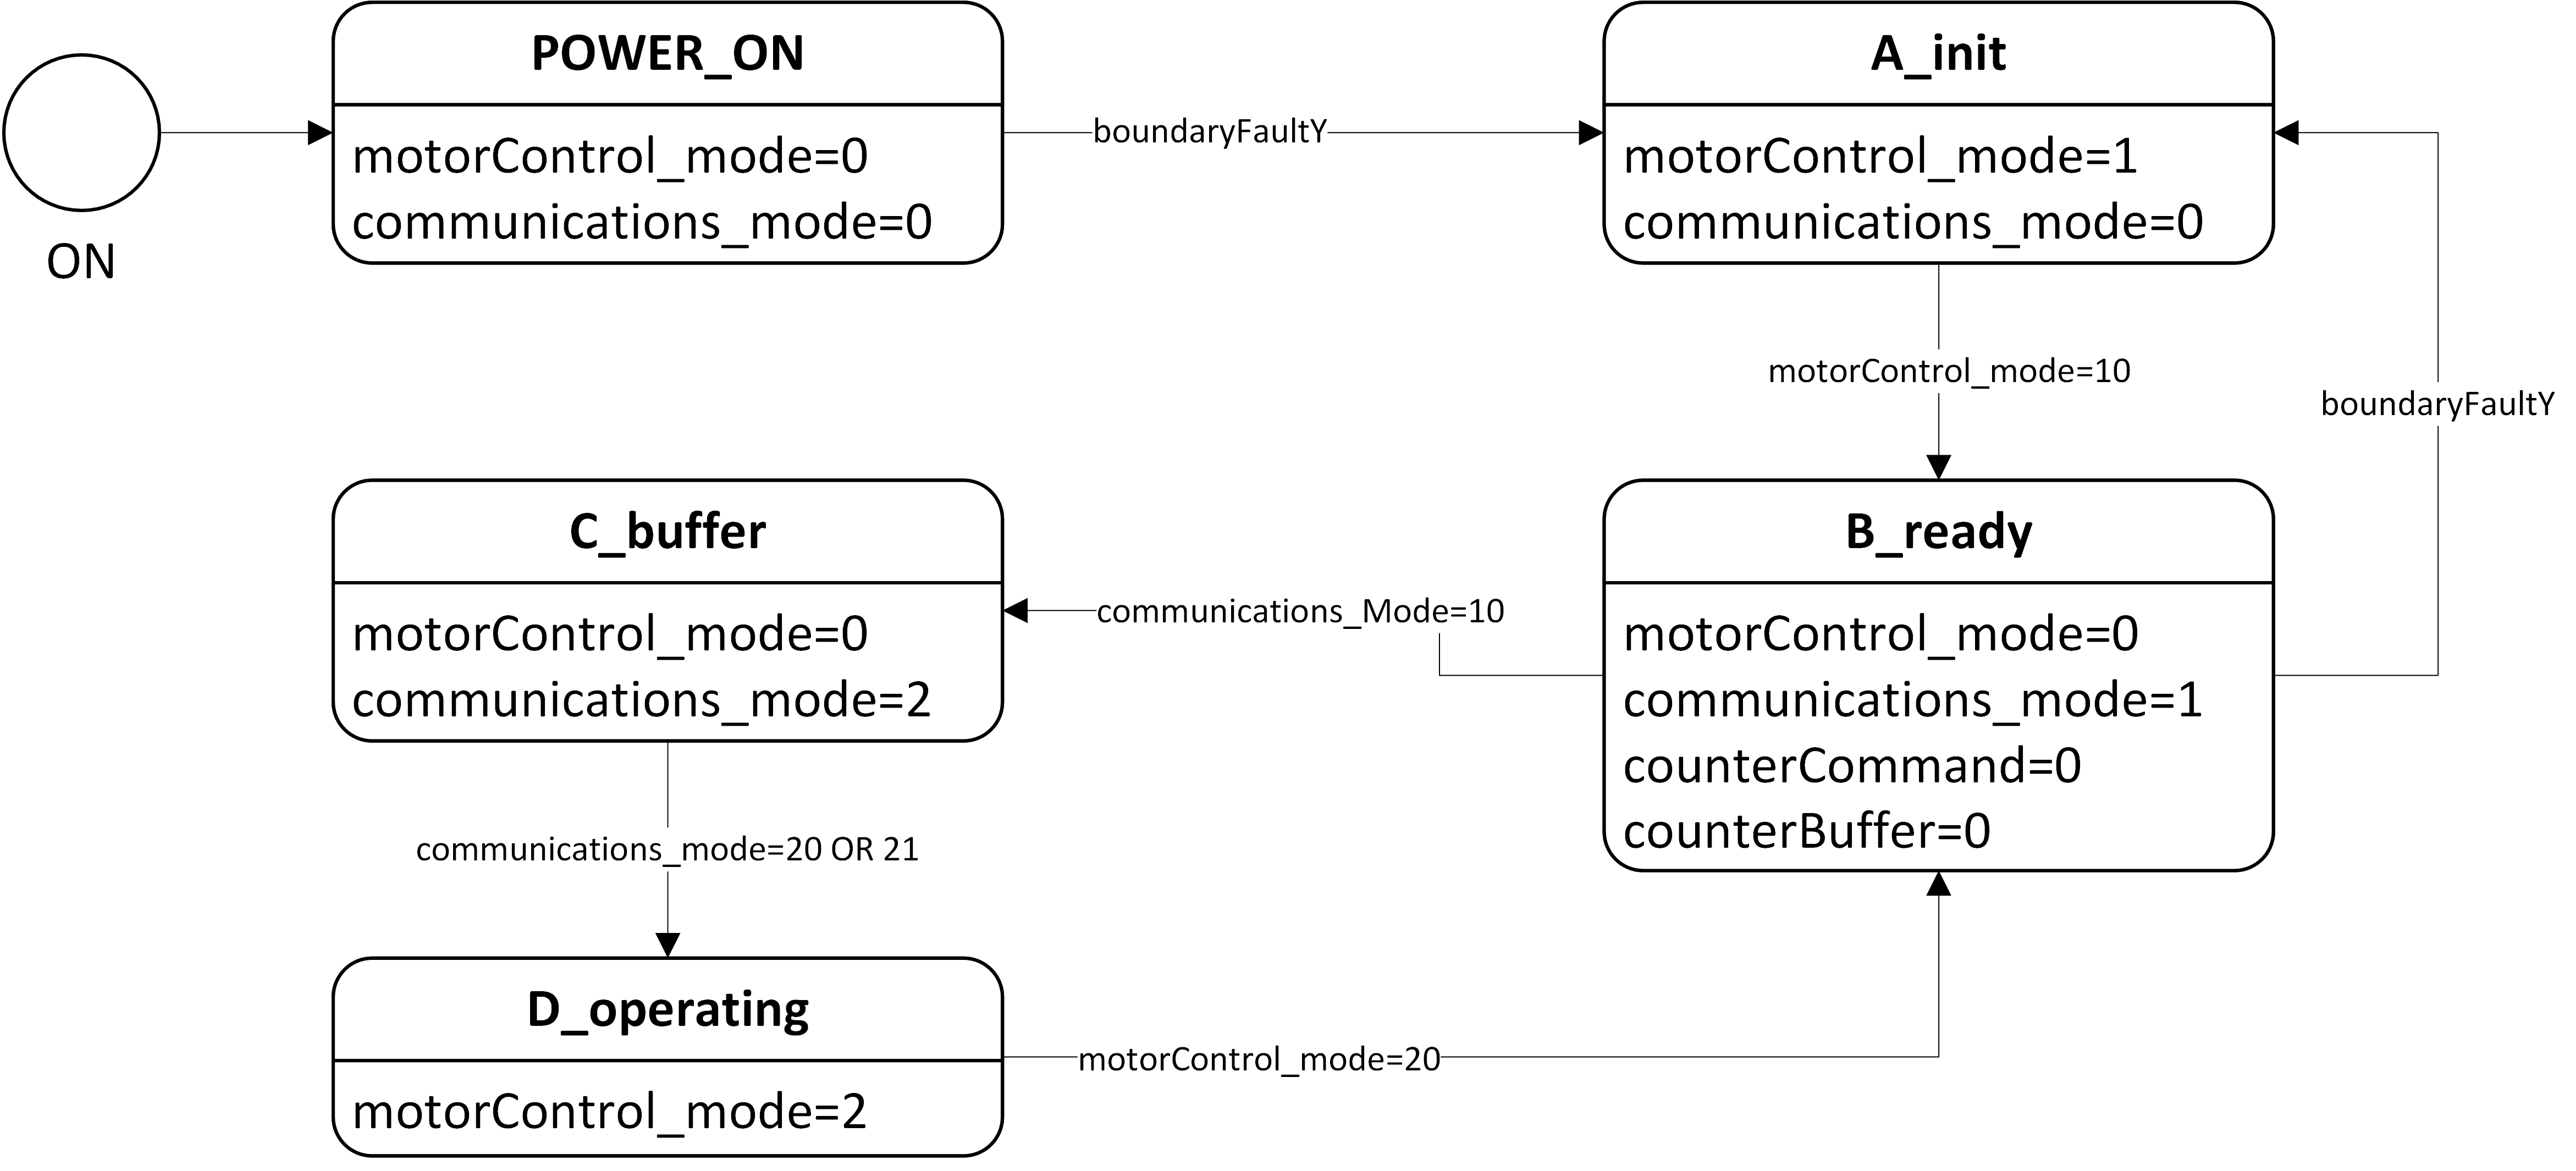
\includegraphics[width=\textwidth]{figures/cncMachine/governor}
				\captionof{figure}{The Governor State Machine}
				\label{fig:PLC-flowcharts-governor}
		\end{center}

\section{Communications State Machine}
\label{sec:PLC-flowcharts-comms}

	\begin{center}
		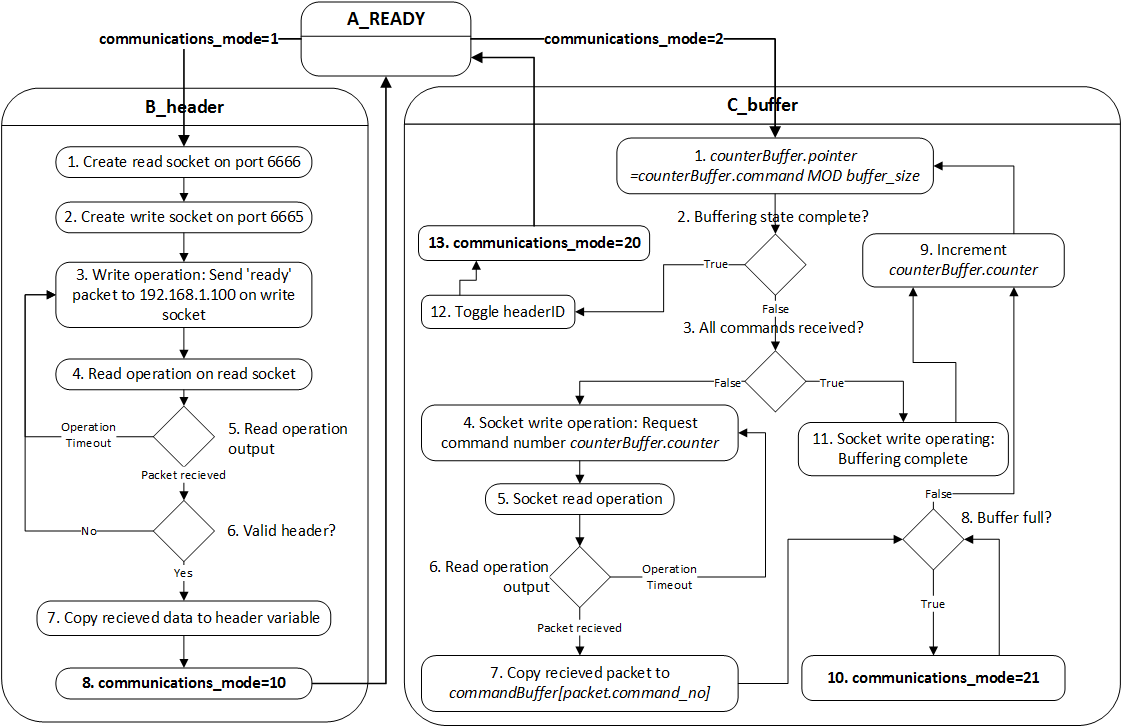
\includegraphics[width=\textwidth]{figures/cncMachine/communications}
		\captionof{figure}{Communications program: States and State Actions}
		\label{fig:communicationsStates}
	\end{center}

\section{motorControl State Machine}
\label{sec:PLC-flowcharts-motor}
	\begin{center}
		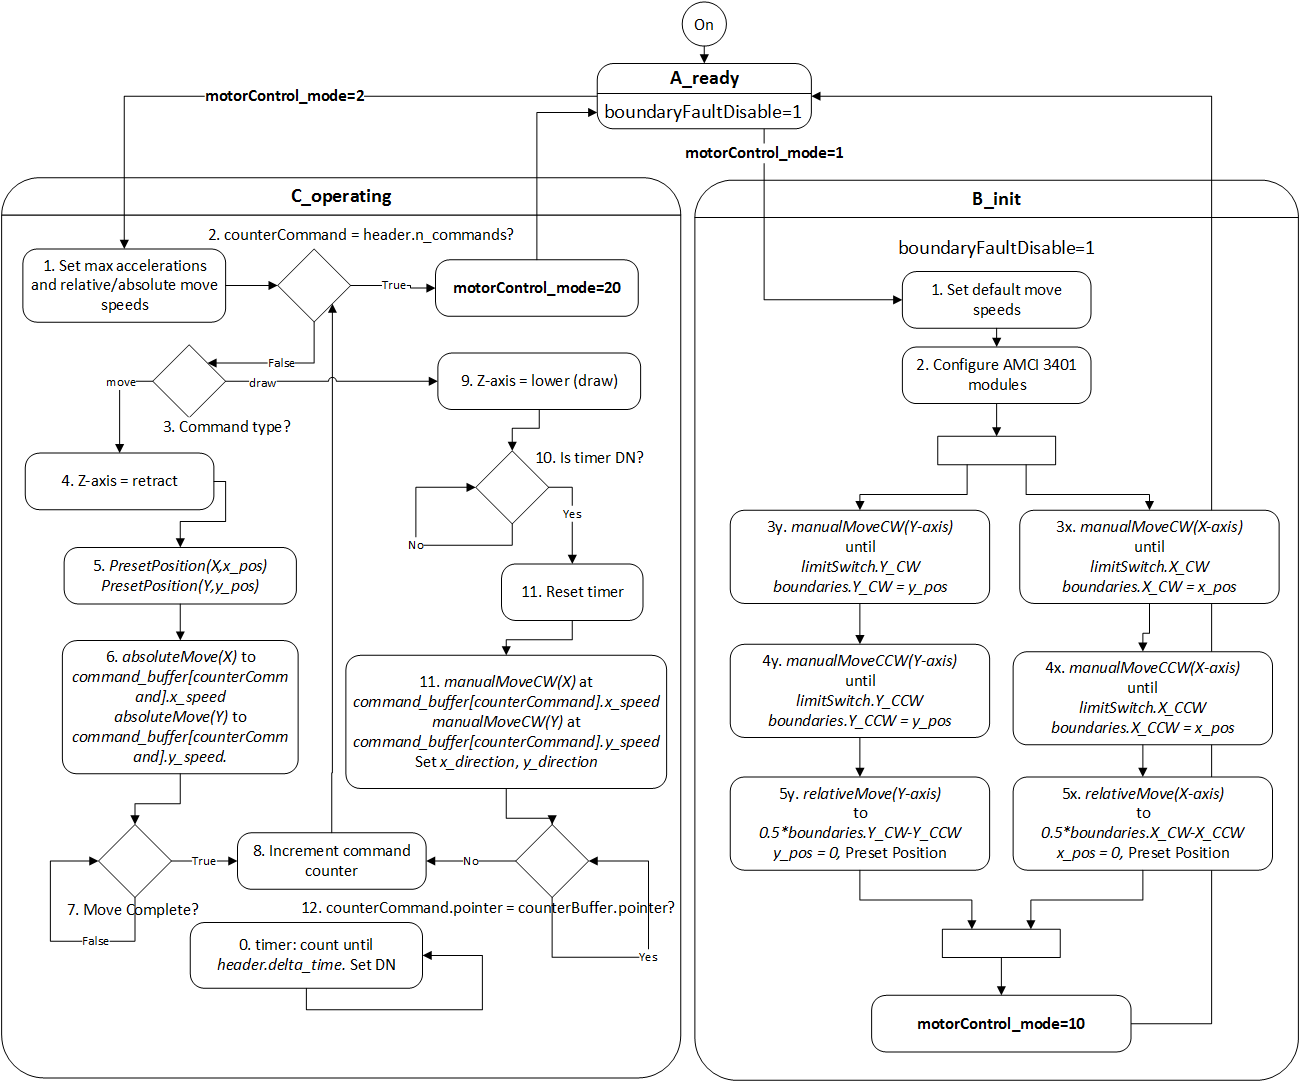
\includegraphics[width=\textwidth]{figures/cncMachine/motorControl}
		\captionof{figure}{motorControl Program: States and State Actions}
		\label{fig:motorControlStates}
	\end{center}

	\subsubsection{Introduction to the AMCI 3401 Stepper Module}
	\label{sec:PLC-flowcharts-amci}
			The main purpose of the motorControl program is to communicate with the two AMCI 3401 Stepper Motor Modules. Their primary role is to send two types of control signals to the stepper motor modules:\\
			\begin{description}
				\item[Step Output] \hfill \\
					A $5V$ square pulse output, with each rising edge signifying a single step of the motor.
				\item[Direction Output] \hfill \\
					A $5V$ boolean output that defines which direction the stepper motors should turn.
			\end{description}
			The modules takes its input by asynchronously monitoring a 16-byte command word on the PLC and mirror it internally. All commands given by the motorControl program involving modifying this command word. \\
			In addition, the module monitors its relative position and operating state by providing a 16-byte status word.\\
			The modules feature a broad range of commands, but the those used by the DoodleBot system are:
			\begin{description}
				\item[Absolute Move] \hfill \\
					Given a position in space (relative to the preset origin position), the AMCI module creates the appropriate velocity profile to get there (within the acceleration/deceleration/top speed parameter limits).
				\item[Relative Move] \hfill \\
					Given a distance to travel (from the current position), the AMCI module creates the appropriate velocity profile to get there (within the acceleration/deceleration/top speed parameter limits).
				\item[Manual Move] \hfill \\
					Manual type moves are actually classified as two separate commands defining the direction of the move  - manual move clockwise, and manual move counterclockwise. These moves accelerate to the programmed speed at the acceleration rate and travel until stopped. While moving in this state, the programmed speed can be changed without having to stop and restart.
				\item[Immediate Stop] \hfill \\
					An immediate stop command stops all current motion.
				\item[Preset Current Position] \hfill \\
					Sets the internal position memory of the module to a position defined in the command word.
			\end{description}

\subsection{Position and Direction Control}
\label{sec:PLC-flowcharts-pos}

	\begin{figure}[htbp!]
		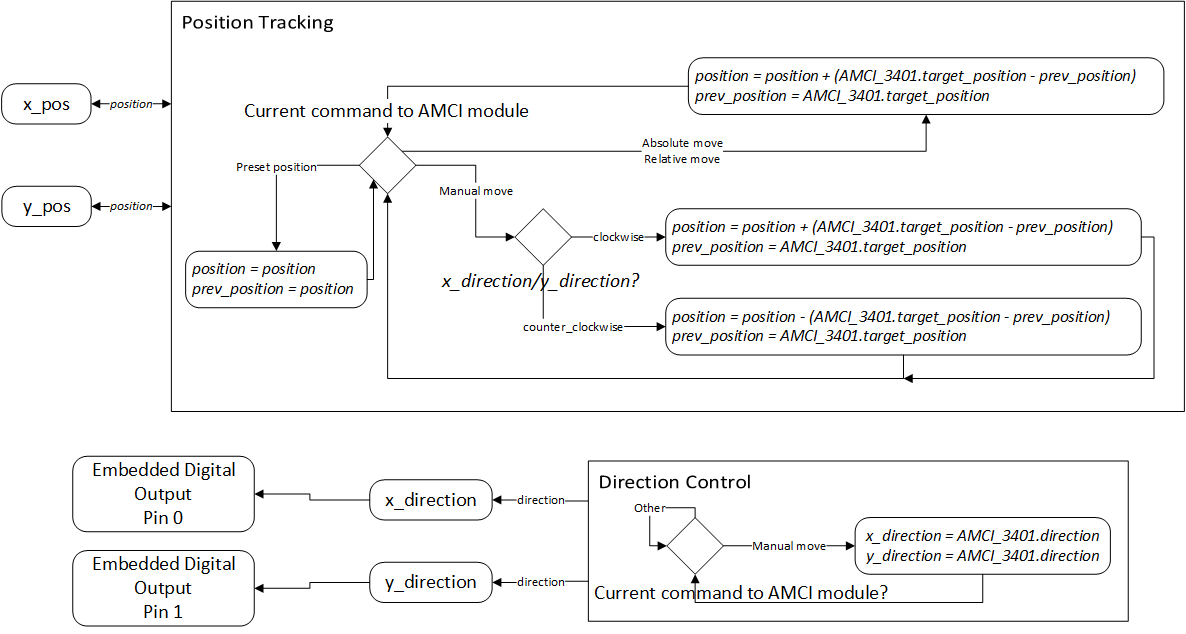
\includegraphics[width=\textwidth]{figures/cncMachine/position_direction}
		\caption{The two routines for managing direction and position}
		\label{fig:Direction and Positional Tracking}
	\end{figure}
	
				\begin{description}
					\item[Absolute Move, Relative Move] \hfill \\
						Relative Moves are treated by the rest of the code as usual. Absolute Moves must be preceded by a Preset Current Position command with the position set to x\_pos and y\_pos. <blah> function monitors the directional state of the AMCI 3401 modules and mirrors this onto the direction output pins. <gah> function measures the change in position since last scan and adds this to x\_pos and y\_pos.
					\item[Manual Move] \hfill \\
						All manual moves, whether clockwise or anticlockwise, are sent to the AMCI 3401 modules as Manual Move Clockwise at the correct speed. The x\_direction and y\_direction bits need to be explicitly set with each Manual Move command to operate in the required direction. Since the AMCI 3401 module thinks it is always moving clockwise (even when it's not), it's internal position state is no longer correct. Function <gah> measures the change in position since last scan and depending on the direction of movement, adds or subtracts this value to x\_pos and y\_pos.
					\item[Preset Current Position] \hfill \\
						Change the value of x\_pos and y\_pos to mirror the position state in the AMCI 3401 controller.
				\end{description}
				
				
	\section{checkLimitSwitch}
	\label{sec:PLC-flowcharts-limit}
		The checkLimitSwitch program is run in a Periodic Task of 10ms and monitors the four limit switches. Upon detecting a rising edge from one of these limit switches, it sets the appropriate boundaryFault value (boundaryFaultX for the X limit switches and boundaryFaultY for the Y limit switches).
		
		If the boundaryFaultDisable is NOT set, it will assume that unintended operation has occurred and an immediate stop command to the stepper motor modules halting all operation. If boundaryFaultDisable IS set then this operation does not happen (used in a situation where motorControl or the Governor are expecting a limit switch input. Eg, boundary checking or waiting for user to manually toggle the switch).
